
\section{Desenvolvimento}
\setlength{\parindent}{2cm}

O projeto se divide em três vertentes principais que são elas: o gerador de clocks, sensor velocidade e o projeto semáforo que serão descritas de maneira detalhada a seguir.

\subsection{Gerador de clocks}
\setlength{\parindent}{2cm}

Nesta etapa usamos comandos sequências para estabelecer todos os clocks que necessitamos no sistema e para tando criamos as seguintes variáveis:\newline

\begin{itemize}
\item \textbf{clk-maquina} - Será o clock automático de frequência de 27MHz 

\item \textbf{temp1, temp0}  - Responsável por definir a temporização especifica para cada clock

temp1 =0 e temp0 = 0 clock da temporização A (Sinal acai e guaraná)

temp1 =0 e temp0 = 1 clock da temporização B (sinal acai e guaraná) 

temp1 =1 e temp0 = 0 clock da temporização C (Sinal acai e guaraná)

\item \textbf{clk-saida-gua,clk-saida-acai }- Após toda logica sequencial for executada isso resultara em dois clocks sendo estes definidos de acordo com a temporização estabelecida.\newline
\end{itemize}

\setlength{\parindent}{2cm}

Para melhor compreensão do gerador temos a simulação de seu seu funcionamento através do waveform, sem as temporizações somente usando o clock automático de 27GHz.
\vskip3ex
\begin{figure}
\centering
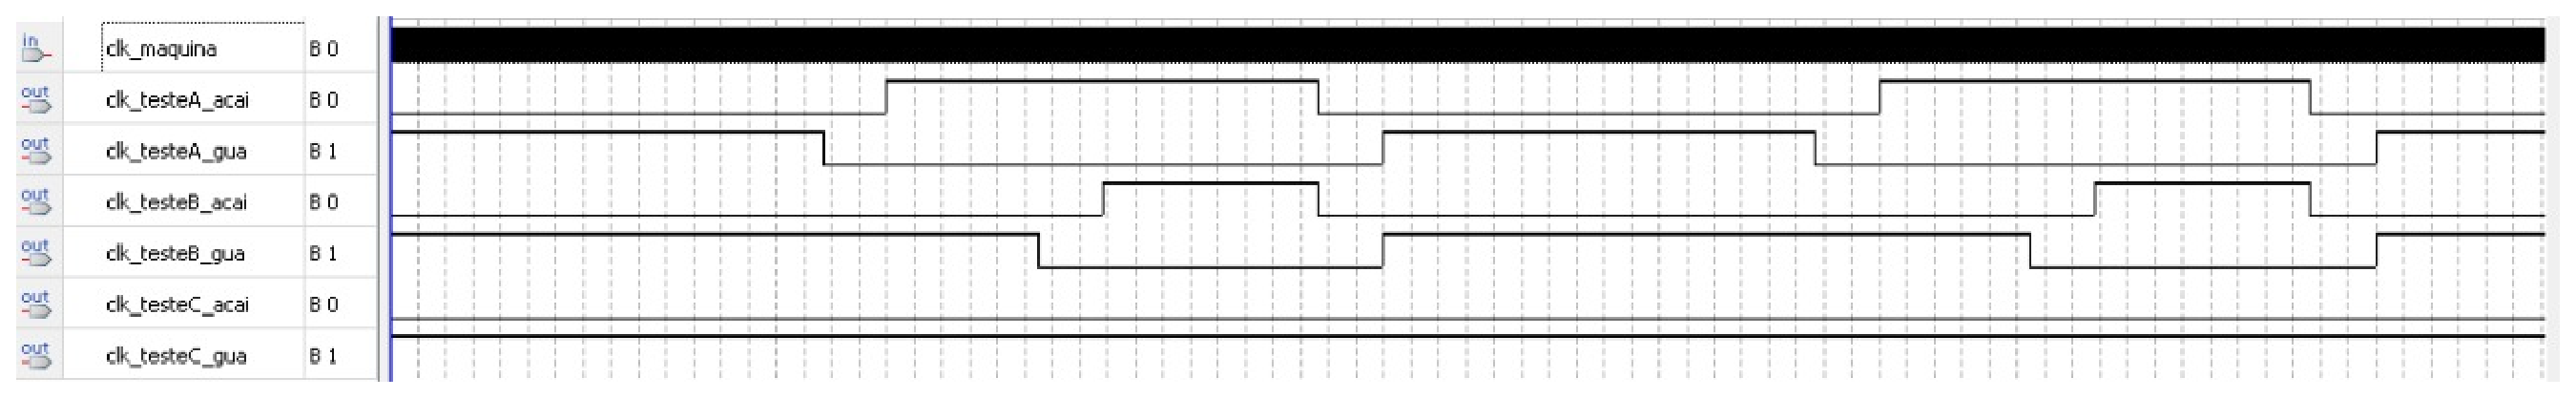
\includegraphics[width=0.99\columnwidth]{clocks.eps}
\end{figure}
\vskip3ex
\setlength{\parindent}{2cm}

obs: Para não haver poluimento visual todo o código se encontrara em anexo.

\subsection{Projeto Semáforo}

\setlength{\parindent}{2cm}

Nesta etapa desenvolvemos o sistema de semáforos, para isto se fez necessário o uso de todos os clocks e dos temporizações, para que com isto conseguíssemos obter as equações lógicas para cada luz do semáforo, tendo para isso o uso das seguintes variáveis.\newline

\begin{itemize}
\item  \textbf{clk-maquina} - Será o clock automático de frequência de 27MHz 
\item \textbf{guarana-vermelho,guarana-amarelo,guarana-verde} - Luzes do sinal guarana
\item \textbf{acai-vermelho,acai-amarelo,acai-verde} - Luzes do sinal acai
\item \textbf{temp1, temp0}  - Temporização de cada sinal \newline
\end{itemize}

\setlength{\parindent}{2cm}
Seguindo com o raciocínio usando na implementação do projeto, usamos o item Gerador de clock anteriormente desenvolvido como componente desta etapa e através da funcionalidade portmap passamos os parâmetros necessários para obter todos os clocks para as três temporizações requisitadas.

Para entender o funcionamento do sistema de forma obsoleta vamos analisar a seguir a simulação no waveform de todos os sinais nas três temporizações que o trabalho estabelece.\newline

Para Temporização A\newline 
\begin{itemize}
\end{itemize}
		\textbf{Sinal açaí}
\begin{itemize}
\item Verde - 20 segundos ativado
\item Amarelo - 3 segundos desativado
\item Vermelho - 20 segundos desativado\newline
\end{itemize}
	\textbf{Sinal guarana }
\begin{itemize}
\item Verde - 20 segundos ativado
\item Amarelo - 3 segundos desativado
\item Vermelho - 20 segundos desativado 
\end{itemize}

\vskip3ex
\begin{figure}
\centering
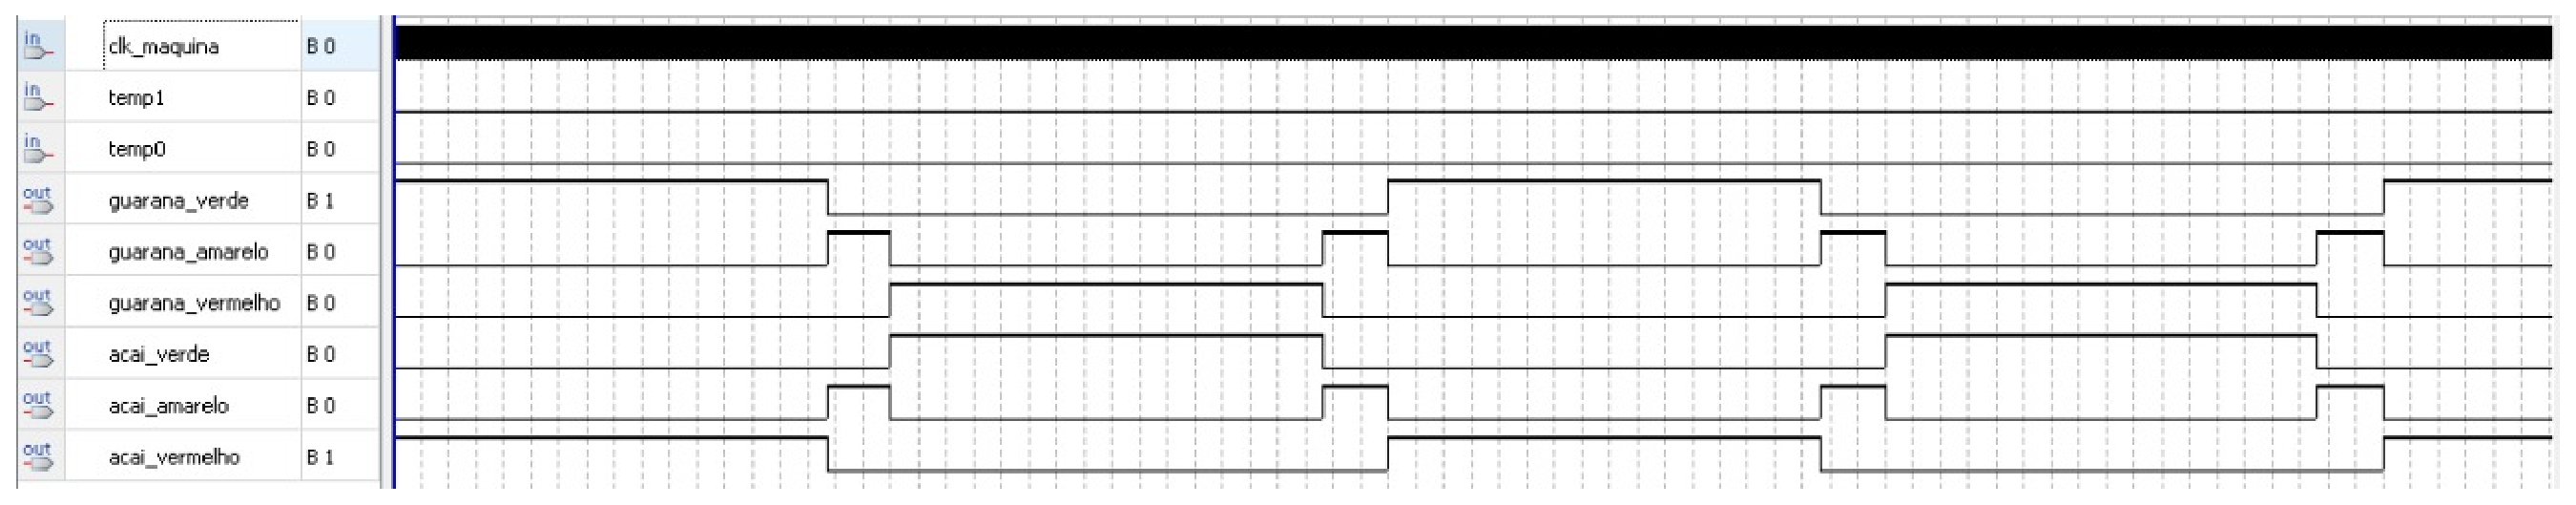
\includegraphics[width=0.99\columnwidth]{temp00.eps}
\end{figure}
\vskip3ex

Para Temporização B\newline 
\begin{itemize}
\end{itemize}
		\textbf{Sinal açaí}
\begin{itemize}
\item Verde - 30 segundos desativado
\item Amarelo - 3 segundos desativado
\item Vermelho - 10 segundos ativado\newline
\end{itemize}
	\textbf{Sinal guarana }
\begin{itemize}
\item Verde - 30 segundos ativado
\item Amarelo - 3 segundos desativado
\item Vermelho - 10 segundos desativado 
\end{itemize}
 

\vskip3ex
\begin{figure}
\centering
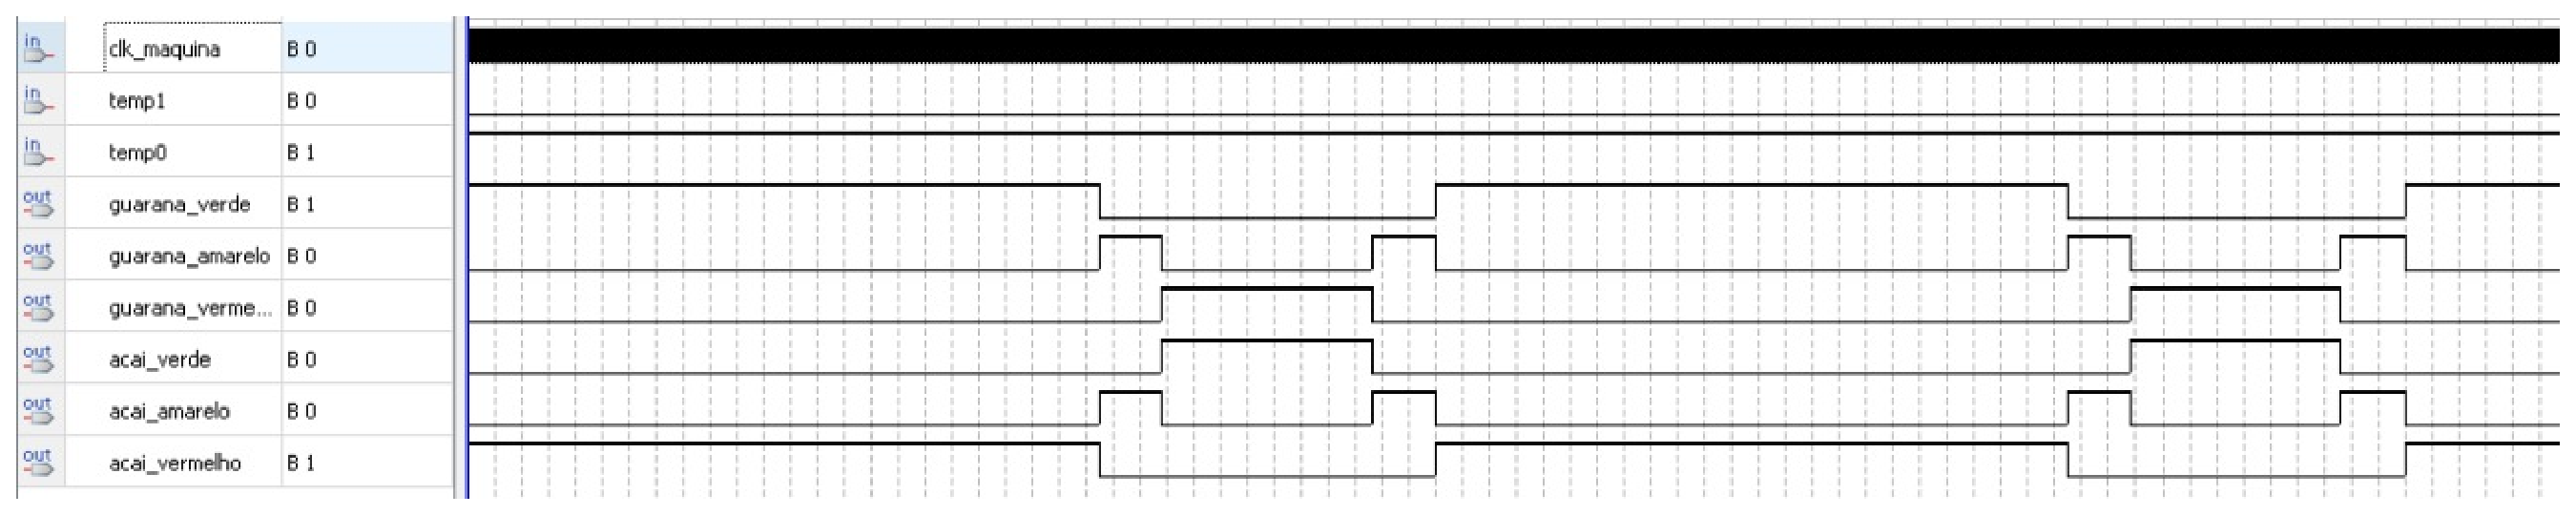
\includegraphics[width=0.99\columnwidth]{temp01.eps}
\end{figure}
\vskip3ex

Para Temporização C\newline 
\begin{itemize}
\end{itemize}
		\textbf{Sinal açaí}
\begin{itemize}
\item O sinal ficara permanentemente neste estado enquanto estiver neste temporizador.
\end{itemize}
	\textbf{Sinal guarana }
\begin{itemize}
\item O sinal ficara permanentemente neste estado enquanto estiver neste temporizador.
\end{itemize}


\vskip3ex
\begin{figure}
\centering
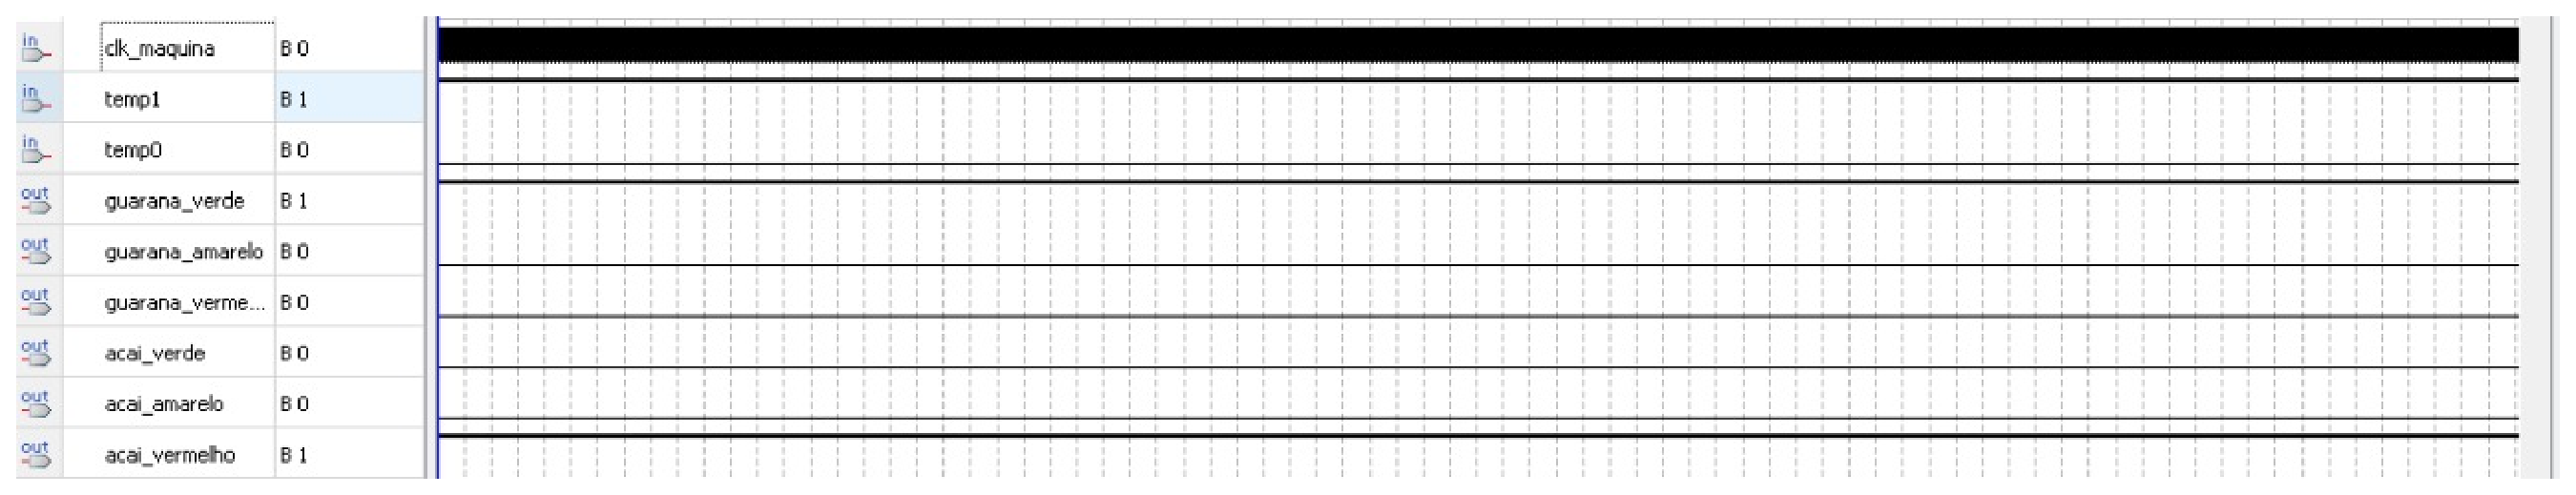
\includegraphics[width=0.99\columnwidth]{temp10.eps}
\end{figure}
\vskip3ex

\setlength{\parindent}{2cm}
Durante toda implementação do trabalho foi decidido que a transição de cada luz do semáforo vai ser feita quando o clock de cada temporização completar seu ciclo. 

\subsection{Sensor de Velocidade}

\setlength{\parindent}{2cm}
Para o sensor de velocidade foi necessário primeiramente a implementação de um contador de 3 segundos, usando para isso o contador desenvolvido no primeiro projeto da disciplina.

Na etapa seguinte estabelecemos as seguintes variáveis:
\begin{itemize}
\item \textbf{clk-maquina} - Será o clock automático de frequência de 27MHz 
\item \textbf{botao1,botao2 } - Controle dos sensores de velocidade (contagem)
\item \textbf{velocidade-ok,velocidade-bad } - Variáveis de saída que dirão se a velocidade ultrapassou o limite exigido.\newline
\end{itmize}


A ideia principal para a execução desta etapa do projeto foi a seguinte: Se o veiculo ultrapassar os 3 segundos (Sinal amarelo) o os sensores de velocidade(botão1 ou botão2) estiverem ativados o veiculo em questão será detectado pelos radares.
\section{Resultados Conclusivos}

\setlength{\parindent}{2cm}
Para conclusão do trabalho o diagrama RTL é mostrado a seguir, onde podemos observar  que os geradores de clock(A,B,C) juntamente com o sensor de velocidade formam o sistema de semáforos ao qual será cadenciado por estes blocos de acordo com a manipulação feita na placa FPGA. 
\vskip3ex
\begin{figure}
\centering
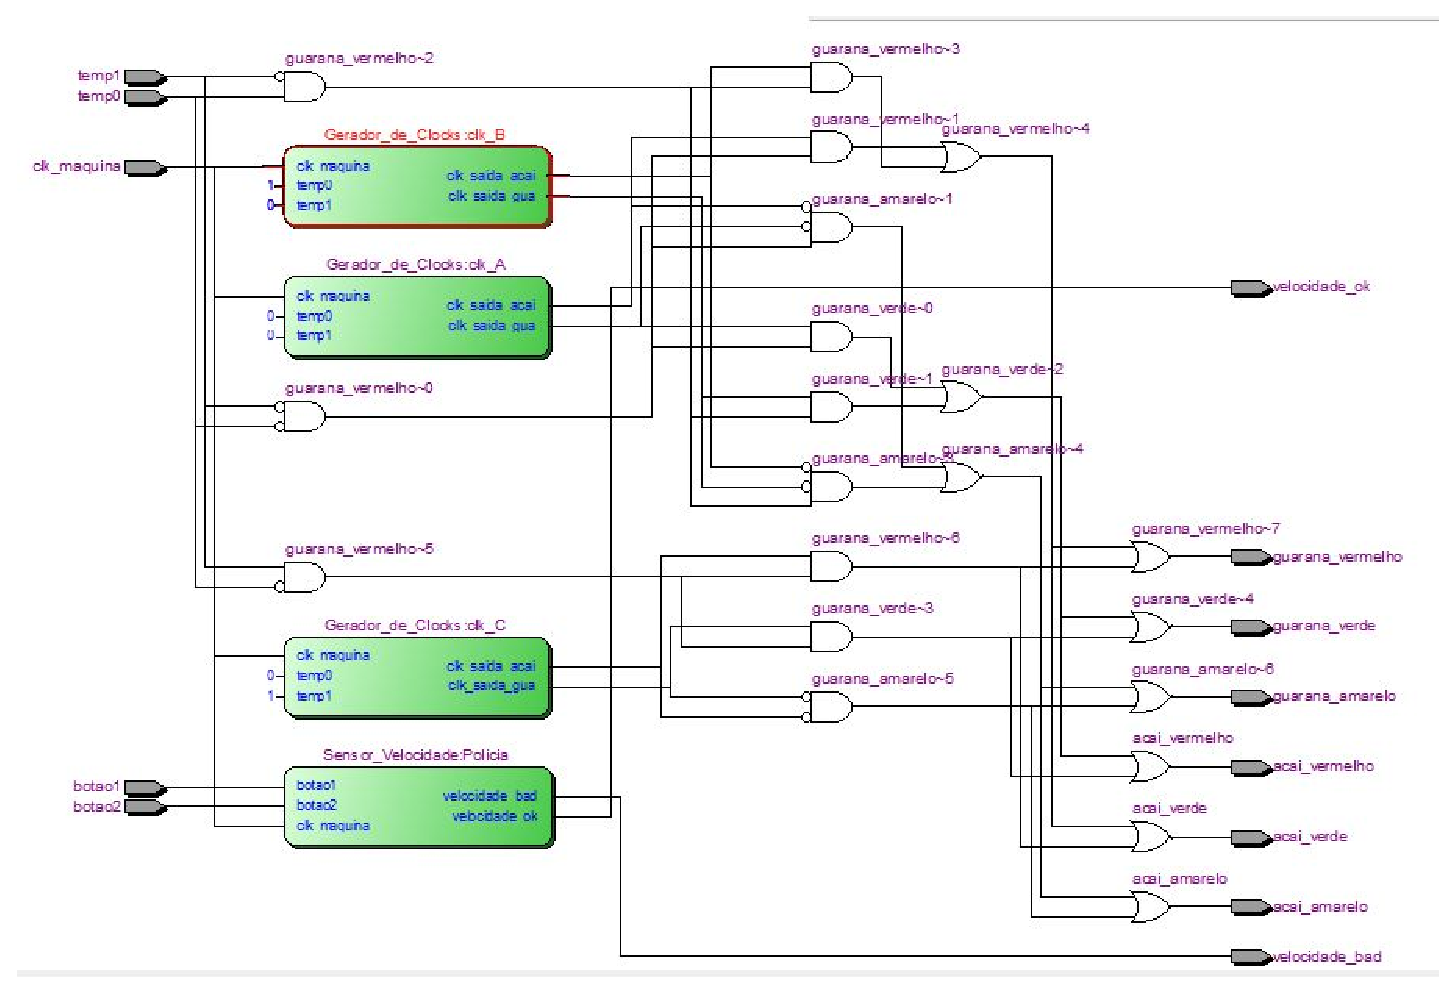
\includegraphics[width=0.99\columnwidth]{rtl.eps}
\end{figure}
\vskip3ex

Todos os códigos implementados bem como o poster poderão ser encontrados no link a seguir:
 \href{https://github.com/mayaracalixta/Poster}{Git Hub}
